%! Author = adnansiddiquei
%! Date = 05/03/2024

% Preamble
\documentclass[a4paper,11pt]{article}
\pdfoutput=1

% Packages
\usepackage{jcappub}
\usepackage[T1]{fontenc}
\usepackage{listings}
\usepackage{roboto}
\usepackage{subcaption}
\usepackage{blindtext}
\usepackage{seqsplit}
\usepackage{booktabs}

%\newcommand{\inlinecode}[1]{\lstinline{#1}}
%\newcommand{\inlinecode}[1]{\texttt{#1}}
\newcommand{\inlinecode}[1]{\texttt{\seqsplit{#1}}}
\lstset{basicstyle=\fontfamily{pcr}\selectfont}


\title{\boldmath Exoplanets: - Coursework Assignment}

% %simple case: 2 authors, same institution
\author{Adnan Siddiquei}
\affiliation{University of Cambridge}

% e-mail addresses: one for each author, in the same order as the authors
\emailAdd{as3438@cam.ac.uk}
\note{Word Count: XXXXX (including figure captions and appendix).}
\bibliographystyle{apalike}

\begin{document}
\maketitle
\flushbottom


%! Author = adnansiddiquei
%! Date = 19/03/2024

\section{Q1}\label{sec:q1}

\clearpage
%! Author = adnansiddiquei
%! Date = 19/03/2024

\section{Q2 - Planet detection and characterisation via RVs}\label{sec:q2}
\subsection{Initial Exploration}\label{subsec:q2-init-exploration}
Radial velocity measurements are extremely useful for detecting exoplanets and characterising their properties.
These measurements are taken by observing the Doppler shift in the spectrum of a star, indicating a shift in the star's velocity
tangential to the observer's line of sight.
However, a variety of stellar "nuisance" signals can also induce these shifts in the star's spectrum.
These include things like oscillations and granulations which occur over the timescales of minutes to hours; rotationally-modulated
activity which occur over the timescale of days to weeks, often in line with the star's rotation period; and magnetic cycles
which are long-term variations in the star's magnetic field.
Likewise, not all periodic signals in the RV data will be due to RV data or stellar signals, it is important to note
that instrument noise or poor sampling (aliasing) can also induce periodic signals in the RV data.

The radial velocity is extracted from an observed spectrum using a cross-correlation function (CCF) which compares the observed
spectrum to a template spectrum of what the star should look like at rest.
From this CCF, two stellar activity indicators can also be extracted: the full width at half maximum (FWHM) and the bisector
span (BIS).
These indicators correlate to the stellar activity signals mentioned above, and can be used to filter out the stellar
activity signals from the radial velocity measurements.

\begin{table}[htb]
    \centering
    \begin{tabular}{ccc}
        \toprule
        \toprule
        Parameter & Units & Value \\
        \midrule
        Rotation Period $P_{rot}$ & days & $31 \pm 10$ \\
        \addlinespace
        Mass $M_{\star}$ & $M_{\odot}$ & $0.69 \pm 0.01$ \\
        \addlinespace
        Effective Stellar Temp. $T_{eff}$ & K & 4500 \\
        \bottomrule
    \end{tabular}
    \caption{Properties of star CB 01223.}
    \label{tab:star_props}
\end{table}

\begin{figure}[htb]
    \centering
    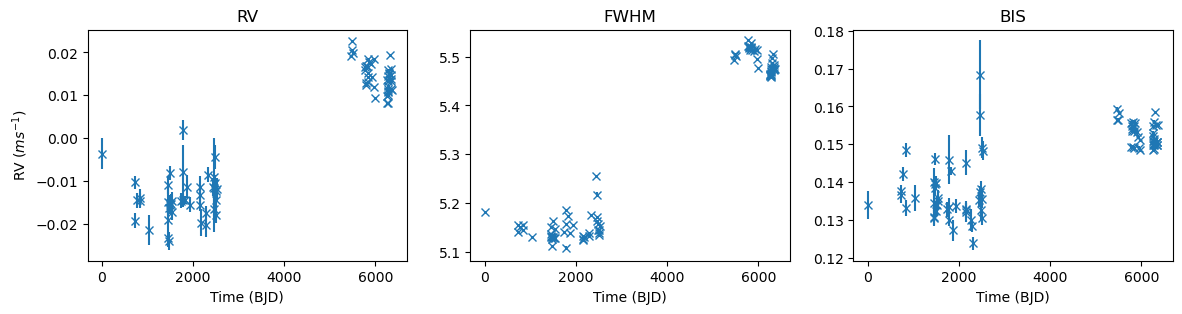
\includegraphics[width=1\textwidth]{figures/data_plot}
    \caption{The radial velocity, FWHM and BIS data for star CB 01223.}
    \label{fig:data_plot}
\end{figure}

Table~\eqref{tab:star_props} shows the properties of the star CB 01223 that this section will analyse and characterise.
Figure~\eqref{fig:data_plot} shows a plot of the RV, FWHM and BIS data for this star.
Initial qualitative inspection of the RV, FWHM and BIS shows a long term correlated positive trend, where all three of the
datasets show a jump in the RV between the two groups of measurements (centered around 2000 BJD and 6000 BJD).
Given the correlation, this indicates that there is a likely long term stellar activity signal present in the data, and given
the time scale, it is likely due to the star's magnetic cycle.

\begin{figure}[htb]
    \centering
    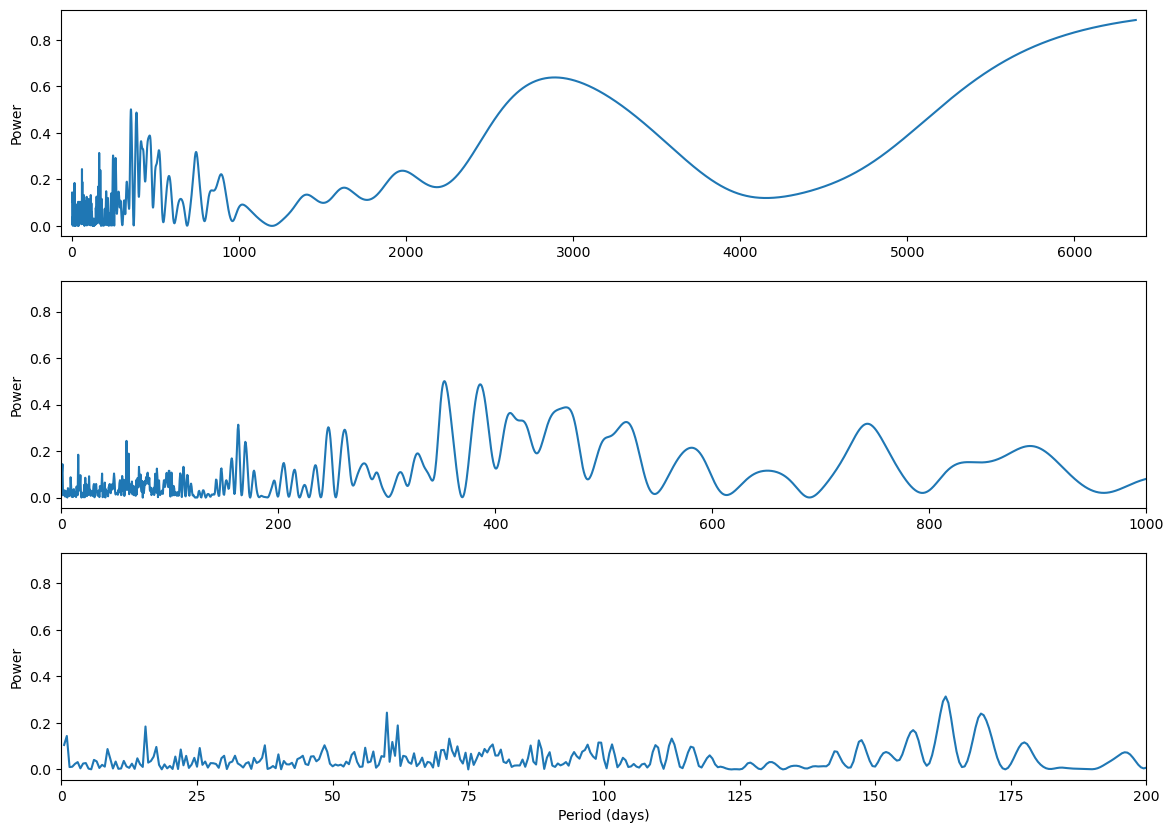
\includegraphics[width=1\textwidth]{figures/lombscargle_periodogram_q2}
    \caption{Lombscargle periodogram of the RV data for star CB 01223. The periodograms are shown at 3 different period
    ranges, with the top plot showing the full range of periods, and the bottom two plots showing zoomed in views of the
    periodogram.}
    \label{fig:lombscargle_periodogram_q2}
\end{figure}

An initial LombScargle periodogram~\cite{lomb, scargle} as shown in Figure~\eqref{fig:lombscargle_periodogram_q2} yields
little useful information.
A peak near the 3000-day mark is likely due to the 2 groups of measurements, and the zoomed in views show no significant
peaks worth exploring.

\subsection{Quantitative Analysis - Evidence of Exoplanets?}\label{subsec:q2-quantitative-analysis}
The exoplanet search conducted in this report follows closely with the methodology used by Faria, et al. (2022)~\cite{faria2022}
to search for exoplanets in the radial velocity data of Proxima Centauri.
They initially utilised a joint RV and FWHM Gaussian process (GP) model to model the stellar activity signals in the data,
and subtracted this from the RV data before fitting a Keplerian model to the residuals.
This methodology is extended slightly and a joint GP model is fit to all three of the RV, FWHM and BIS datasets to model
the stellar activity.

\begin{equation}\label{eq:qp-kernel}
    \mathcal{K}_{\text{QP}}(\tau) =
    \theta_1^2 \exp
    \left[
        -\frac{\tau^2}{2 \theta_2^2} - \frac{\sin^2 \left( \frac{\pi |t_{i} - t_{j}|}{\theta_3} \right)}{\theta_4^2}
    \right]
\end{equation}

Equation \eqref{eq:qp-kernel} shows the Quasi-Periodic (QP) kernel used in the GP model, where all $\theta_{2}, \theta_{3}
\theta_{4}$ were all shared between the RV, FWHM and BIS datasets (hence the joint GP model), but $\theta_{1}$ was allowed
to float for each dataset.

\begin{table}[htb]
    \centering
    \begin{tabular}{ccc}
        \toprule
        \toprule
        Parameter & Units & Prior \\
        \midrule
        Amplitude $\theta_{1}$ RV & $ms^{-1}$ & $\mathcal{U}(1e^{-4}, 3 \Delta$RV$)$ \\
        \addlinespace
        Amplitude $\theta_{1}$ FWHM & $ms^{-1}$ & $\mathcal{U}(1e^{-4}, 3 \Delta$FWHM$)$  \\
        \addlinespace
        Amplitude $\theta_{1}$ BIS & $ms^{-1}$ & $\mathcal{U}(1e^{-4}, 10 \Delta$BIS$)$ \\
        \addlinespace
        Exp Length Scale $\theta_{2}$ & $s$ & $\mathcal{U}(1e^{-4}, 3 \Delta$t$)$ \\
        \addlinespace
        Stellar Period $\theta_{3}$ & $s$ & $\mathcal{G}(31, 10)$ \\
        \addlinespace
        Periodic Length Scale $\theta_{4}$ & $s$ & $\mathcal{U}(1e^{-4}, 3 \Delta$t$)$ \\
        \addlinespace
        Jitter $j$ & $ms^{-1}$ & $\mathcal{LU}(1e^{-10}, 1e^{-6})$ \\
        \bottomrule
    \end{tabular}
    \caption{Parameters and priors for the joint QP GP model on the RV, FWHM and BIS datasets.
    $\mathcal{U}(a, b)$ denotes a uniform prior between $a$ and $b$; $\mathcal{G}(\mu, \sigma)$ denotes a Gaussian prior
    with mean $\mu$ and standard deviation $\sigma$; and $\mathcal{LU}(a, b)$ denotes a log-uniform prior between $a$ and $b$.}
    \label{tab:stellar_gp_priors}
\end{table}

Table~\eqref{tab:stellar_gp_priors} shows a list of all the parameters and priors used for the joint stellar activity
GP model.
Note that the data was standardised before fitting the GP model to help with convergence, the table lists the priors
in the non-standardised scale, but these were converted to the standardised scale before fitting.
Bringing the data to a common scale also allowed for a single jitter term to be used across all three datasets, reducing
the number of parameters that needed to be fit.
In general, relatively uninformative priors were used for all the parameters, all priors covered a multiple of the entire
extent of their respective data.

A Markov Chain Monte Carlo (MCMC) simulation was then run, drawing initial samples from these priors with 250 walkers and
2000 iterations per walker.
Samples were extracted with a burn in of 100 iterations and a thinning factor of 20 to reduce autocorrelation.
Figure~\eqref{fig:stellar_noise_corner_plot} shows the corner plot of this MCMC simulation, and
Figure~\eqref{fig:stellar_noise_fit} shows the GP model fit to the RV, FWHM and BIS datasets from the maximum likelihood
sample of the MCMC simulation.

\begin{figure}[htb]
    \centering
    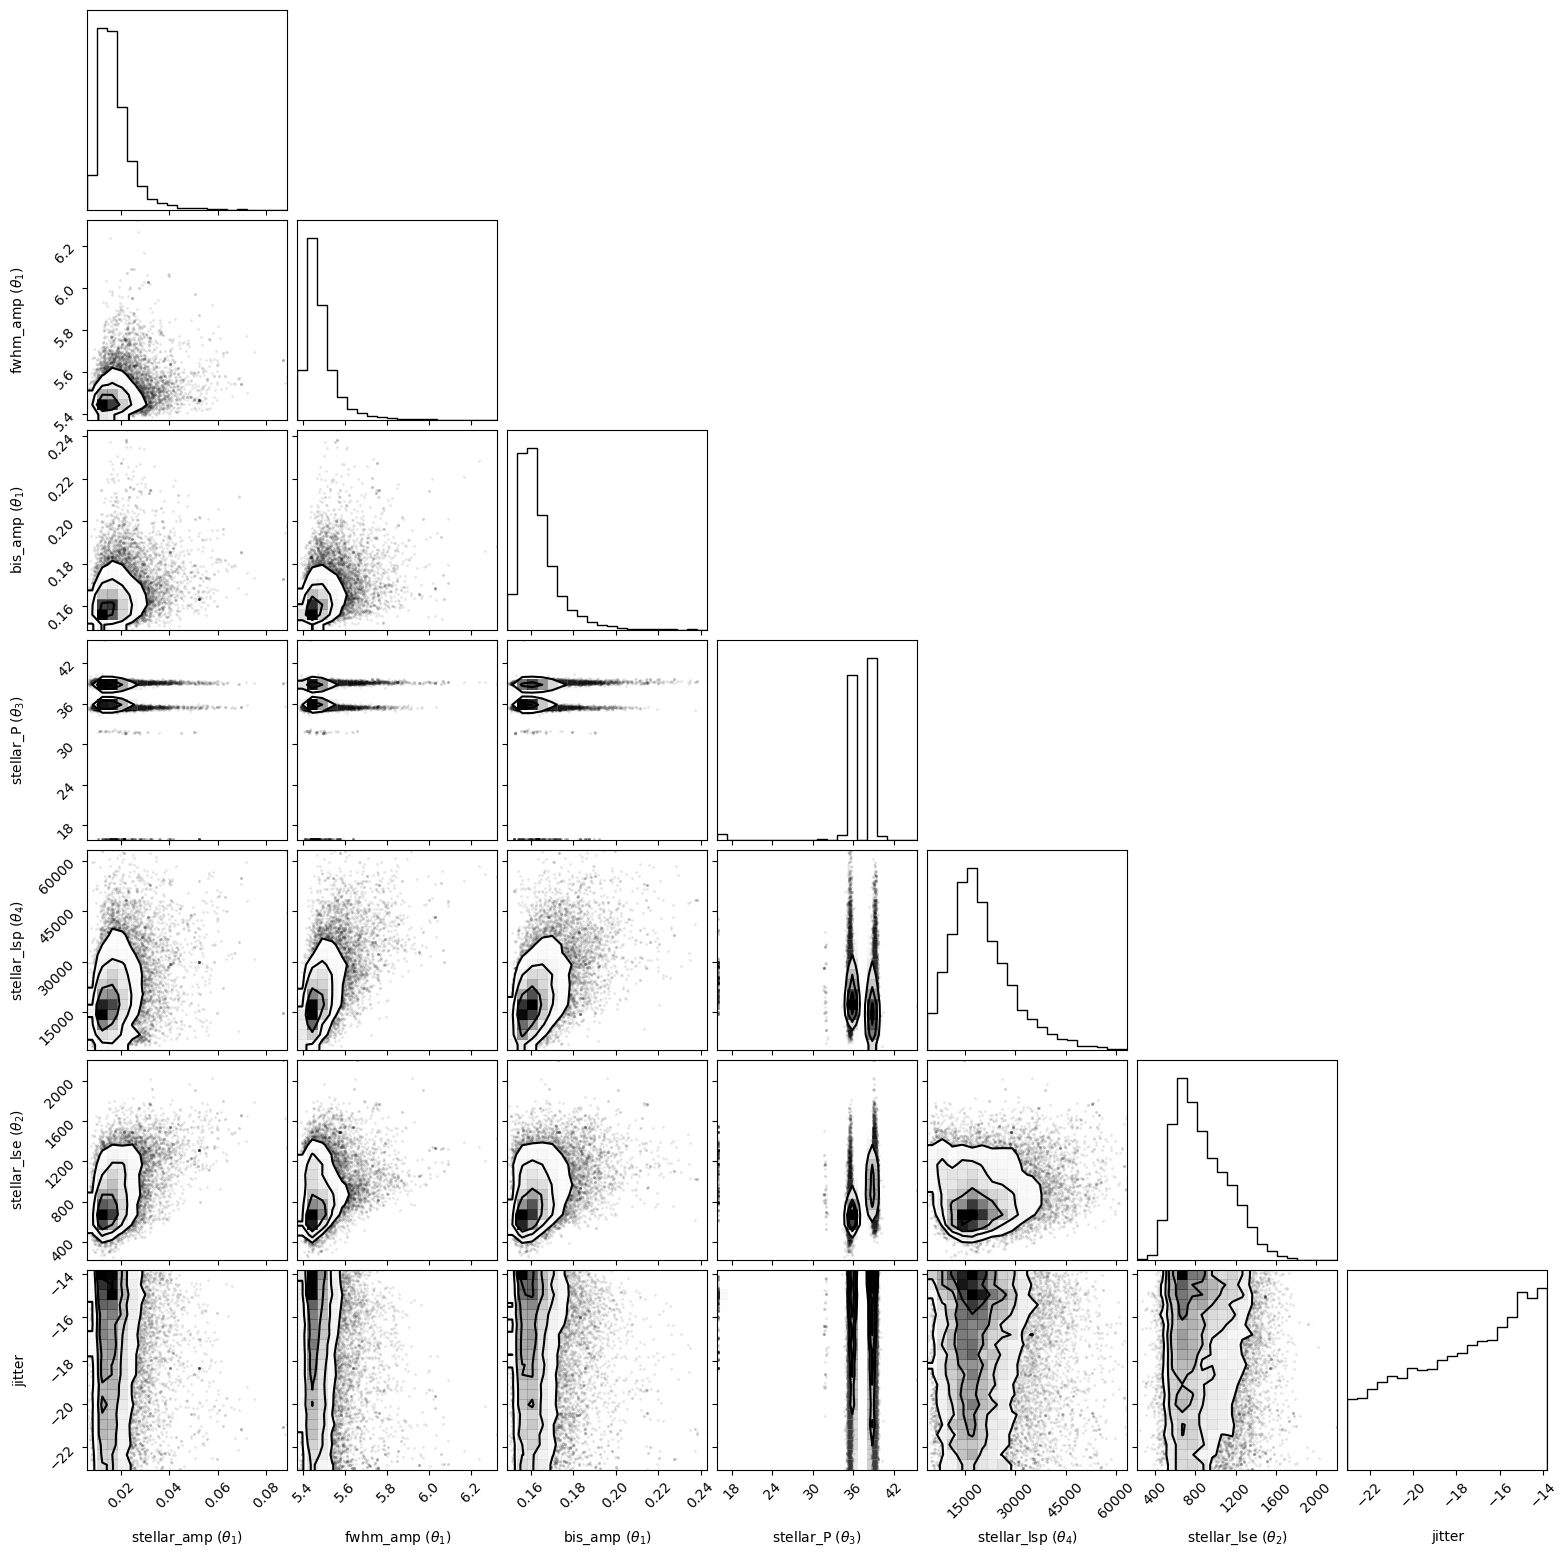
\includegraphics[width=1\textwidth]{figures/stellar_noise_corner_plot}
    \caption{}
    \label{fig:stellar_noise_corner_plot}
\end{figure}

\begin{figure}[htb]
    \centering
    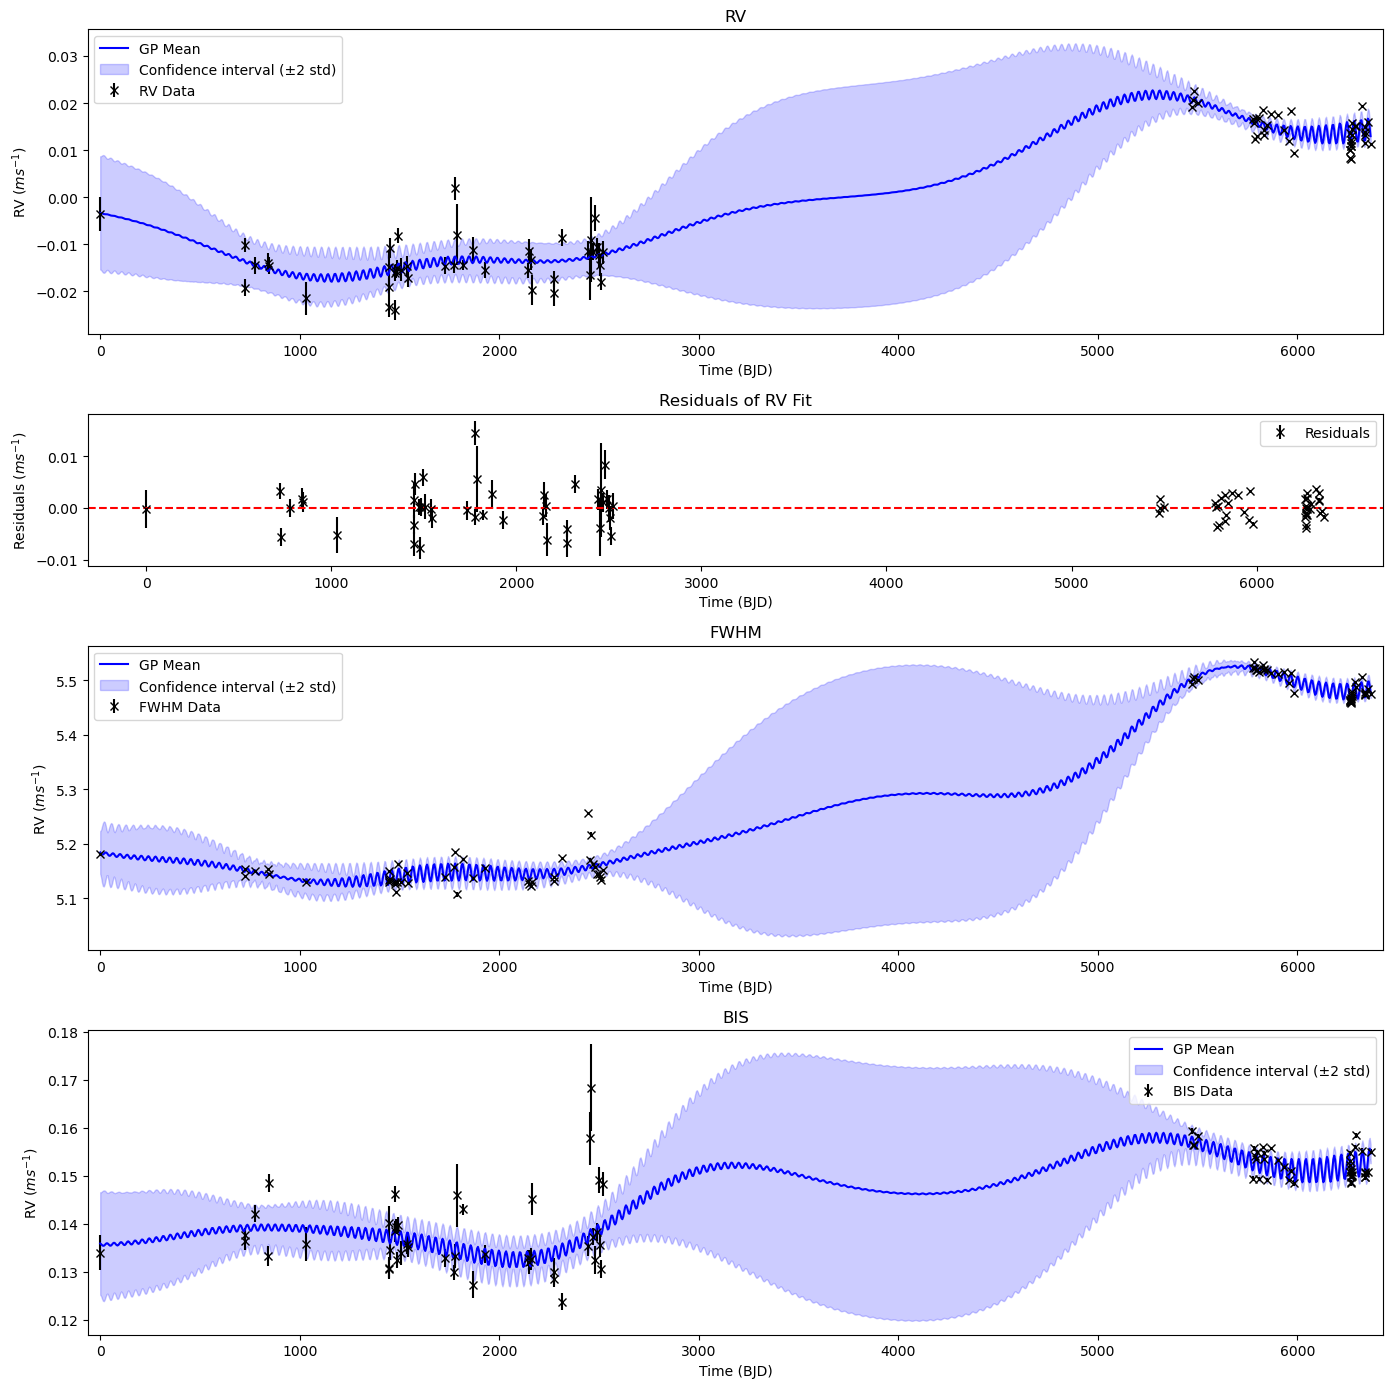
\includegraphics[width=1\textwidth]{figures/stellar_noise_fit}
    \caption{The GP model fit to the RV, FWHM and BIS datasets for star CB 01223.
    The central purple lines show the maximum likelihood fit from the MCMC simulation, and the shaded regions show the
    2$\sigma$ confidence intervals.
    The second plot shows the residuals of the GP model fit to the RV data.}
    \label{fig:stellar_noise_fit}
\end{figure}


\clearpage
\appendix

%\section{MNIST Classifier Details}\label{app:mnist-classifier}
%The MNIST classifier model is a CNN composed of 4 \inlinecode{CNNBlocks} ($[32, 64, 128, 64]$ channels per block) followed by an
%\inlinecode{nn.AdaptiveAvgPool2d} to lower the dimensionality of the penultimate feature vector to 1024 before it is fed into
%a fully connected \inlinecode{nn.Linear} layer with 10 output units (one for each class in the MNIST dataset).
%This classifier was trained for 21 epochs with a batch size of 128 and a learning rate of $2 \times 10^{-4}$ using the Adam optimiser.
%The loss function used was the cross-entropy loss function and the test set classification accuracy reached was 99.34\% on
%the final epoch.
%To extract the 1024-length feature vector, the final \inlinecode{nn.Linear} layer was set to \inlinecode{nn.Identity}
%so that the model outputted the penultimate layer feature vector instead of the class predictions.
%The model was trained on the MNIST training set and the test set was used for evaluation of the FMD.

\begin{thebibliography}{99}

    \bibitem{hippke2019}
    Hippke, M., and Heller, R.,
    \textit{Transit Least Squares: Optimized transit detection algorithm to search for periodic transits of small planets}.
    arXiv preprint arXiv:1901.02015, 2019.
    Available at \url{https://arxiv.org/abs/1901.02015} [Accessed: 20-Jun-2024].

    \bibitem{lomb}
    Lomb, N.R.,
    \textit{Least-squares frequency analysis of unequally spaced data}.
    Astrophysics and Space Science, 39(2), pp.447-462, 1976.
    Available at \url{https://doi.org/10.1007/BF00648343} [Accessed: 20-Jun-2024].

    \bibitem{scargle}
    Scargle, J.D.,
    \textit{Studies in astronomical time series analysis. II - Statistical aspects of spectral analysis of unevenly spaced data}.
    The Astrophysical Journal, 263, pp.835-853, 1982.
    Available at \url{https://doi.org/10.1086/160554} [Accessed: 20-Jun-2024].

    \bibitem{faria2022}
    Faria, J.P., Suárez Mascareño, A., Figueira, P., et al.,
    \textit{A candidate short-period sub-Earth orbiting Proxima Centauri}.
    Astronomy \& Astrophysics, 658, A115, 2022.
    Available at \url{https://doi.org/10.1051/0004-6361/202142337} [Accessed: 20-Jun-2024].


\end{thebibliography}



\end{document}
